\begin{figure}
    \centering
    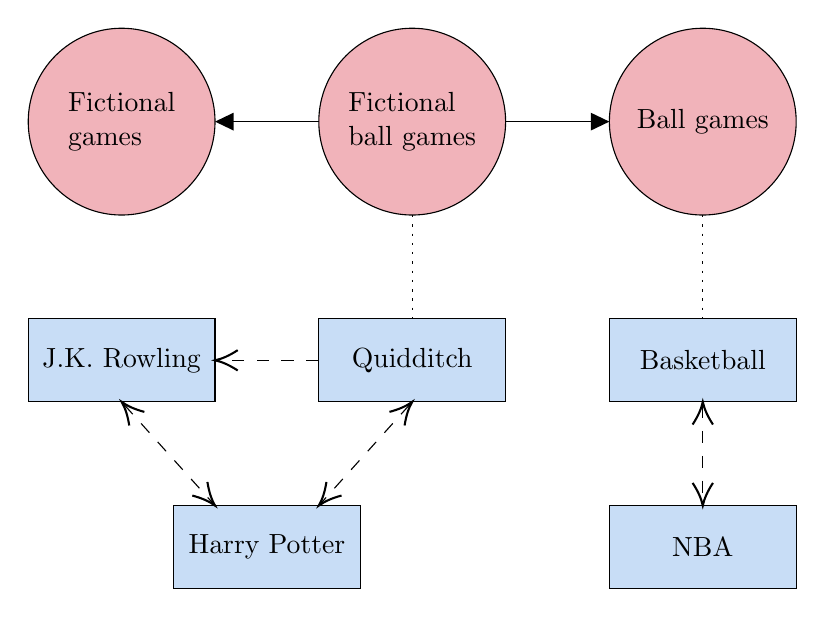
\begin{tikzpicture}[x=0.75pt,y=0.75pt,yscale=-1,xscale=1]
        %Shape: Circle [id:dp8115219034229394] 
        \draw  [fill={rgb, 255:red, 208; green, 2; blue, 27 }  ,fill opacity=0.3 ] (10,55) .. controls (10,30.15) and (30.15,10) .. (55,10) .. controls (79.85,10) and (100,30.15) .. (100,55) .. controls (100,79.85) and (79.85,100) .. (55,100) .. controls (30.15,100) and (10,79.85) .. (10,55) -- cycle ;
        %Shape: Circle [id:dp8163711353091557] 
        \draw  [fill={rgb, 255:red, 208; green, 2; blue, 27 }  ,fill opacity=0.3 ] (150,55) .. controls (150,30.15) and (170.15,10) .. (195,10) .. controls (219.85,10) and (240,30.15) .. (240,55) .. controls (240,79.85) and (219.85,100) .. (195,100) .. controls (170.15,100) and (150,79.85) .. (150,55) -- cycle ;
        %Shape: Circle [id:dp9514147881884653] 
        \draw  [fill={rgb, 255:red, 208; green, 2; blue, 27 }  ,fill opacity=0.3 ] (290,55) .. controls (290,30.15) and (310.15,10) .. (335,10) .. controls (359.85,10) and (380,30.15) .. (380,55) .. controls (380,79.85) and (359.85,100) .. (335,100) .. controls (310.15,100) and (290,79.85) .. (290,55) -- cycle ;
        %Straight Lines [id:da26929607637664343] 
        \draw    (150,55) -- (102,55) ;
        \draw [shift={(100,55)}, rotate = 360] [fill={rgb, 255:red, 0; green, 0; blue, 0 }  ][line width=0.75]  [draw opacity=0] (8.93,-4.29) -- (0,0) -- (8.93,4.29) -- cycle    ;
        
        %Straight Lines [id:da55975302746763] 
        \draw    (240,55) -- (288,55) ;
        \draw [shift={(290,55)}, rotate = 180] [fill={rgb, 255:red, 0; green, 0; blue, 0 }  ][line width=0.75]  [draw opacity=0] (8.93,-4.29) -- (0,0) -- (8.93,4.29) -- cycle    ;
        
        %Shape: Rectangle [id:dp5695294519694281] 
        \draw  [fill={rgb, 255:red, 74; green, 144; blue, 226 }  ,fill opacity=0.3 ] (150,150) -- (240,150) -- (240,190) -- (150,190) -- cycle ;
        %Shape: Rectangle [id:dp9459907669998763] 
        \draw  [fill={rgb, 255:red, 74; green, 144; blue, 226 }  ,fill opacity=0.3 ] (10,150) -- (100,150) -- (100,190) -- (10,190) -- cycle ;
        %Shape: Rectangle [id:dp9118915462525985] 
        \draw  [fill={rgb, 255:red, 74; green, 144; blue, 226 }  ,fill opacity=0.3 ] (80,240) -- (170,240) -- (170,280) -- (80,280) -- cycle ;
        %Shape: Rectangle [id:dp706551589936829] 
        \draw  [fill={rgb, 255:red, 74; green, 144; blue, 226 }  ,fill opacity=0.3 ] (290,150) -- (380,150) -- (380,190) -- (290,190) -- cycle ;
        %Shape: Rectangle [id:dp23087103101225726] 
        \draw  [fill={rgb, 255:red, 74; green, 144; blue, 226 }  ,fill opacity=0.3 ] (290,240) -- (380,240) -- (380,280) -- (290,280) -- cycle ;
        %Straight Lines [id:da05502265811536389] 
        \draw  [dash pattern={on 4.5pt off 4.5pt}]  (150,170) -- (102,170) ;
        \draw [shift={(100,170)}, rotate = 360] [color={rgb, 255:red, 0; green, 0; blue, 0 }  ][line width=0.75]    (10.93,-4.9) .. controls (6.95,-2.3) and (3.31,-0.67) .. (0,0) .. controls (3.31,0.67) and (6.95,2.3) .. (10.93,4.9)   ;
        
        %Straight Lines [id:da5354993058131741] 
        \draw  [dash pattern={on 4.5pt off 4.5pt}]  (193.66,191.49) -- (151.34,238.51) ;
        \draw [shift={(150,240)}, rotate = 311.99] [color={rgb, 255:red, 0; green, 0; blue, 0 }  ][line width=0.75]    (10.93,-4.9) .. controls (6.95,-2.3) and (3.31,-0.67) .. (0,0) .. controls (3.31,0.67) and (6.95,2.3) .. (10.93,4.9)   ;
        \draw [shift={(195,190)}, rotate = 131.99] [color={rgb, 255:red, 0; green, 0; blue, 0 }  ][line width=0.75]    (10.93,-4.9) .. controls (6.95,-2.3) and (3.31,-0.67) .. (0,0) .. controls (3.31,0.67) and (6.95,2.3) .. (10.93,4.9)   ;
        %Straight Lines [id:da11087403714951327] 
        \draw  [dash pattern={on 4.5pt off 4.5pt}]  (56.34,191.49) -- (98.66,238.51) ;
        \draw [shift={(100,240)}, rotate = 228.01] [color={rgb, 255:red, 0; green, 0; blue, 0 }  ][line width=0.75]    (10.93,-4.9) .. controls (6.95,-2.3) and (3.31,-0.67) .. (0,0) .. controls (3.31,0.67) and (6.95,2.3) .. (10.93,4.9)   ;
        \draw [shift={(55,190)}, rotate = 48.01] [color={rgb, 255:red, 0; green, 0; blue, 0 }  ][line width=0.75]    (10.93,-4.9) .. controls (6.95,-2.3) and (3.31,-0.67) .. (0,0) .. controls (3.31,0.67) and (6.95,2.3) .. (10.93,4.9)   ;
        %Straight Lines [id:da7909762012355506] 
        \draw  [dash pattern={on 4.5pt off 4.5pt}]  (335,192) -- (335,238) ;
        \draw [shift={(335,240)}, rotate = 270] [color={rgb, 255:red, 0; green, 0; blue, 0 }  ][line width=0.75]    (10.93,-4.9) .. controls (6.95,-2.3) and (3.31,-0.67) .. (0,0) .. controls (3.31,0.67) and (6.95,2.3) .. (10.93,4.9)   ;
        \draw [shift={(335,190)}, rotate = 90] [color={rgb, 255:red, 0; green, 0; blue, 0 }  ][line width=0.75]    (10.93,-4.9) .. controls (6.95,-2.3) and (3.31,-0.67) .. (0,0) .. controls (3.31,0.67) and (6.95,2.3) .. (10.93,4.9)   ;
        %Straight Lines [id:da5382710413033004] 
        \draw  [dash pattern={on 0.84pt off 2.51pt}]  (195,100) -- (195,150) ;
        
        %Straight Lines [id:da6347712182350267] 
        \draw  [dash pattern={on 0.84pt off 2.51pt}]  (335,100) -- (335,150) ;
        
        % Text Node
        \draw (55,55) node  [align=left] {Fictional\\games};
        % Text Node
        \draw (195,55) node  [align=left] {Fictional\\ball games};
        % Text Node
        \draw (335,55) node  [align=left] {Ball games};
        % Text Node
        \draw (195,170) node  [align=left] {Quidditch};
        % Text Node
        \draw (335,260) node  [align=left] {NBA};
        % Text Node
        \draw (125,260) node  [align=left] {Harry Potter};
        % Text Node
        \draw (55,170) node  [align=left] {J.K. Rowling};
        % Text Node
        \draw (335,170) node  [align=left] {Basketball};
    \end{tikzpicture}
    \caption{Example of an extended semantic graph, as presented in \cite{Bonetti}. Blue nodes represent the semantic graph of Wikipedia articles --- the so-called \textquote{Wikigraph} \cite{Buriol} --- and red nodes represent the taxonomy-like structure of Wikipedia categories --- the so-called Wikipedia Category Graph (WCG) \cite{Zesch}. These two graphs can be merged thanks to the fact that each Wikipedia article can be linked to a number of categories. Edges drawn in dissimilar styles model different semantic relations between nodes.}
    \label{extended_semantic_graph}
\end{figure}